\documentclass{article}
\usepackage[utf8]{inputenc}
\usepackage[T1]{fontenc}
\usepackage{graphicx}
\usepackage{hyperref}
\usepackage{geometry}
\geometry{margin=1in}

\title{AMIGALLE}
\date{Encyclopaedia Britannica (1771)}

\begin{document}
\maketitle

\section*{Historical source}
\textbf{Entry ID:} \texttt{entry-amigalle-560} \\
\textbf{Volume ID:} 191253801 \\
\textbf{Character Count:} 1079

\subsection*{Extracted Text}
AMIGALLE, in a general lenic, denotes any thing done in a friendly manner, or to promote peace.

\_Ancare Bruder,\_ Roman majority, were, according to Prifice, lower and lets honourable feats al-lotted for the \_judica redenia\_, or inferior judges, who upon being admitted of the emperor's council, were dig- nished by him with the title \_amisi\_.

\_Ancare Number,\_ such are mutually equal to the ten of one another’s aliquipur parts. Thus the numbers 284 and 230 are amicable numbers : for the alt- parparts 1, 2, 4, 5, 19, 11, 20, 23, 44, 55, 110, of 220, are targeted equal to each other than 284 ‡ and the aliquipur parts 1, 2, 4, 71, 142, of 284, are together equal to 230.

AMCTUS in Roman antiquity, was any upper garment worn over the tunics.

Asarrers, among octahedral writers, the uppermost garment warranty worn by the clergy : the other five being the alba, fingellum, foda, mangalo, and plauso. The amefter was a linem garment, of a spare papers, covering the head, rocks, and houlders, and buckled or chipel before the breath. It is still worn by the religious abroad.



\section*{Source record}
\begin{itemize}
\item \textbf{Dataset:} \texttt{NationalLibraryOfScotland/encyclopaedia\_britannica\_illustrated}
\item \textbf{Dataset Revision:} \texttt{309f765b1ecc83e0a7f7762e44b4a927a7555443}
\item \textbf{Page ID:} \texttt{britannica:309f765b1ecc83e0a7f7762e44b4a927a7555443:train:560} \\
  \textbf{Filename:} \texttt{page-0560-c458f594fc79.jpg} \\
  \textbf{Row Index:} 560 \\
  \textbf{SHA256:} \texttt{c458f594fc79392e...}
\end{itemize}

\begin{figure}[h]
\centering
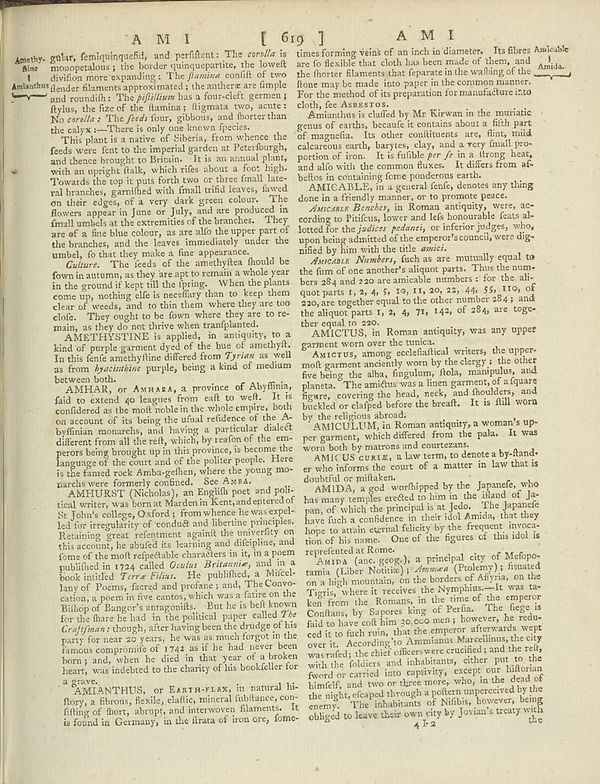
\includegraphics[width=0.85\textwidth]{../scans/page-0560-c458f594fc79.jpg}
\caption*{Source scan: \texttt{page-0560-c458f594fc79.jpg}}
\end{figure}

\end{document}
